\documentclass[
  12pt,
  openright,
  twoside,
  a4paper,
  english,
  brazil
]{abntex2}

% Configurações de pacotes utilizados

\usepackage{lmodern}
\usepackage[T1]{fontenc}
\usepackage[utf8]{inputenc}
\usepackage{lastpage}
\usepackage{indentfirst}
\usepackage{color}
\usepackage{graphicx}
\usepackage{adjustbox}
\usepackage{microtype}
\usepackage[brazilian, hyperpageref]{backref}
\usepackage[alf]{abntex2cite}
\renewcommand{\backrefpagesname}
\renewcommand{\backref}{}
\renewcommand*{\backrefalt}[4]{}

% Dados para capa e folha de rosto

\titulo{Desenvolvimento de Aplicações em Java e\\Utilizando Conceitos de UI e UX}
\autor{Pedro Felipe Froes Silva}
\local{Belo Horizonte}
\data{2017}
\orientador{Kecia Aline Marques Ferreira}
\coorientador{Avenue Code Desenvolvimento e Comércio de Softwares Ltda}
\instituicao{
  Centro Federal de Educação Tecnológica de Minas Gerais
  \par
  Departamento de Computação
  \par
  Curso de Engenharia de Computação
}
\tipotrabalho{Relatório}
\preambulo{Relatório apresentado ao Curso de Engenharia de Computação do Centro Federal de Educação Tecnológica de Minas Gerais, como requisito parcial para a aprovação na disciplina Estágio Supervisionado.}

% Configurações do PDF gerado

\definecolor{blue}{RGB}{41,5,195}
\makeatletter
\hypersetup{
  pdftitle={\@title},
	pdfauthor={\@author},
  pdfsubject={\imprimirpreambulo},
  pdfcreator={LaTeX with abnTeX2},
	pdfkeywords={estágio supervisionado}{java}{ui}{ux},
	colorlinks=true,
  linkcolor=blue,
  citecolor=blue,
  filecolor=magenta,
  urlcolor=blue,
  bookmarksdepth=4
}
\makeatother
\setlength{\parindent}{1.3cm}
\setlength{\parskip}{0.2cm}
\interfootnotelinepenalty=10000

% Inclusão de seções do trabalho

\makeindex
\begin{document}
\frenchspacing
\imprimircapa
\imprimirfolhaderosto*

%\begin{fichacatalografica}
%\end{fichacatalografica}

%\begin{folhadeaprovacao}
%	\begin{center}
%		Espaço destinado à folha de aprovação
%	\end{center}
%\end{folhadeaprovacao}

%\begin{dedicatoria}
%	\vspace*{\fill}
%	\centering
%	\noindent
%	\textit{Dedicatória a ser escrita.} \vspace*{\fill}
%\end{dedicatoria}

%\begin{agradecimentos}
%	Agradecimentos a serem escritos.
%\end{agradecimentos}

%\setlength{\absparsep}{18pt}

%\begin{resumo}
%	Resumo a ser escrito.
%	\textbf{Palavras-chave}: Meta-design. \textit{Design system}. Linguagem de domínio específico. DSL.
%\end{resumo}

%\begin{resumo}[Abstract]
%	\begin{otherlanguage*}{english}
%    	Abstract to be written.
%		\textbf{Keywords}: Meta-design. Design system. Domain-specific language. DSL.
%	\end{otherlanguage*}
%\end{resumo}

%\pdfbookmark[0]{\listfigurename}{lof}
%\listoffigures*
%\cleardoublepage

%\pdfbookmark[0]{\listtablename}{lot}
%\listoftables*
%\cleardoublepage

%\begin{siglas}
%	\item[CAD] Desenho Assistido por Computador (\textit{Computer Aided Design})
%	\item[CSS] Folhas de Estilo em Cascata (\textit{Cascading Style Sheets})
%	\item[DSL] Linguagem de domínio específico (\textit{domain specific language})
%	\item[GPL] Linguagem de propósito geral (\textit{general purpose language})
%	\item[HTML] Linguagem de Marcação de Hipertexto (\textit{Hyper Text Markup Language})
%\end{siglas}

\pdfbookmark[0]{\contentsname}{toc}
\tableofcontents*
\cleardoublepage

\textual
\chapter{Introdução}
\label{cap:introducao}

O presente trabalho é um relatório da disciplina de Estágio Supervisionado pertencente ao curso de Engenharia de Computação do Centro Federal de Educação Tecnológica de Minas Gerais (CEFET-MG), realizado pelo discente Pedro Felipe Froes na empresa Avenue Code Desenvolvimento e Comércio de Software Ltda. Este relatório reflete o período de Março a Maio de 2017 durante o estágio do aluno na empresa, contemplando parte do Programa de Estágio Jedi Internship.

O Programa de Estágio Jedi Internship da Avenue Code corresponde a uma rotação dos participantes por diferentes tecnologias presentes na área de Computação. Durante o período do programa, o estagiário passa por cinco áreas distintas, obtendo um aprendizado de linguagens de programação como (i) Java e (ii) Ruby, (iii) do \textit{framework} .NET, (iv) de conceitos de garantia de qualidade de software, e (v) de conceitos e \textit{frameworks} para o desenvolvimento de interfaces de usuário (\textit{user interface}, UI). O estudante exercita o aprendizado de cada área por meio de projetos internos da empresa, e apresenta um \textit{workshop} com o conteúdo aprendido ao final de cada etapa.

O objetivo desse trabalho é relatar as experiências do discente nas áreas em que o mesmo participou durante o período do Estágio Supervisionado, que correspondem ao aprendizado de Java e de conceitos de UI. O aprendizado em cada uma das áreas é apresentado por meio do processo de desenvolvimento de um migrador de banco de dados em Java e da construção de interfaces de usuário por meio de \textit{frameworks} de UI.

O restante desse trabalho está organizado de forma que o Capítulo~\ref{cap:estagio-supervisionado} apresenta a empresa e o seu Programa de Estágio, enquanto o Capítulo~\ref{cap:fundamentacao-teorica} aponta conceitos básicos de Java e de UI. O Capítulo~\ref{cap:atividades-desenvolvidas} detalha as atividades em cada uma das áreas, enquanto o Capítulo~\ref{cap:conclusao} conclui o trabalho.

\chapter{Estágio supervisionado}
\label{cap:estagio-supervisionado}

Neste capítulo, a empresa concedente Avenue Code e o Programa de Estágio Jedi Internship são apresentados. Tópicos envolvendo a história, especialidade e iniciativas da empresa, bem como a estrutura do programa de estágio são ilustrado nas seções a seguir.

\section{Sobre a empresa: Avenue Code}
\label{sec:sobre-a-empresa}

A Avenue Code Desenvolvimento e Comércio de Softwares Ltd é uma empresa consultora de softwares especializada no ramo de \textit{e-commerce} da indústria varejista. Fundada em 2008 pelo CEO Zeo Solomon na cidade de San Francisco (Califórnia, Estados Unidos da América), a Avenue Code atendia clientes americanos, abrindo seu primeiro escritório no Brasil somente um ano depois, na cidade de Belo Horizonte. Nos anos seguintes, a empresa expande e inaugura um escritório na cidade de São Paulo, além de adicionar Amir Razmara e Chase Hill ao time de CEOs. Em 2017, a Avenue Code é formada por mais de 230 consultores em sua equipe, além de inaugurar um quarto escritório, agora na cidade de Nova York~\cite{ac-who-we-are-2017}.

A Avenue Code é especialista no desenvolvimento e utilização de diversos tipos de tecnologias da área de Computação, como aplicações Web e móveis, automação de infraestruturas, sistemas de \textit{backend}, implementações de plataformas, \textit{coaching} Agile e DevOps e integrações corporativas. A Metodologia Ágil, oriunda do Manifesto Ágil para o Desenvolvimento de Software~\cite{agile-2001}, é altamente aplicada na empresa, que busca maximizar sua eficiência através da utilização de princípios Agile no desenvolvimento de projetos~\cite{ac-what-we-do-2017}.

Prezando tanto pela qualidade da tecnologia utilizada quanto pelo ambiente de trabalho dos consultores, a Avenue Code possui uma gama de empresas parceiras e de prêmios obtidos em sua história. Dentre as empresas de tecnologia parceiras da Avenue Code, figuram a Mulesoft~\footnote{MuleSoft: Integration platform for connecting SaaS and enterprise applications. Disponível em: \url{https://www.mulesoft.com/}}, SAP Hybris~\footnote{SAP Hybris: E-commerce solutions. Disponível em: \url{https://www.hybris.com/en/}}, CHEF~\footnote{Chef: automate IT infrastructure. Disponível em: \url{https://www.chef.io/chef/}}, Oracle~\footnote{Oracle: Integrated cloud applications and platform services. Disponível em: \url{https://www.oracle.com/}}, Amazon Web Services~\footnote{Amazon Web Services (AWS): Cloud computing services. Disponível em: \url{https://aws.amazon.com/}} e Adobe~\footnote{Adobe: Creative, marketing and document management solutions. Disponível em \url{www.adobe.com/}}~\cite{ac-partners-2017}. Já entre os prêmios conquistados pela empresa, estão o reconhecimento pelo LoveMondays~\footnote{Love Mondays: A empresa ideal, avaliada por profissionais como você. Disponível em: \url{https://www.lovemondays.com.br/}}, InfoMoney~\footnote{InfoMoney: Notícias, ações e muito mais sobre investimentos. Disponível em: \url{www.infomoney.com.br/}} e San Francisco Business Times's Fast 100~\footnote{San Francisco Business Time Fast 100. Disponível em: \url{http://www.bizjournals.com/sanfrancisco/blog/2016/10/bay-area-fast-growing-private-companies-fast-100.html}} em 2016, além de ser agraciada como uma das Melhores Empresas para Trabalhar~\footnote{Great Place to Work. Disponível em: \url{www.greatplacetowork.com.br/}} em 2016 (\textit{Great Place to Work})~\cite{ac-who-we-are-2017}.

Por fim, a Avenue Code participa de iniciativas de inclusão digital por meio do programa AC Social, que oferta aulas de introdução à tecnologias e computação em escolas carentes. A empresa também oferece cursos ministrados pelos próprios consultores por meio do AC Community, além de ofertar dois programas de estágios distintos, o AC Wonder Women e o Jedi Internship, que será apresentado na seção seguinte~\cite{ac-academy-2017}.

\section{Sobre o estágio: Programa de Estágio Jedi Internship}
\label{sec:sobre-o-estagio}

O Programa de Estágio Jedi Internship consiste de uma rotação (\textit{job rotation}) por cinco áreas de diferentes tecnologias presentes na área de Computação. São elas:

\begin{itemize}
	\item Conceitos e \textit{frameworks} de \textit{user interface} (UI) e \textit{user experience} (UX)
	\item Conceitos e \textit{frameworks} de garantia de qualidade de software
	\item Linguagem de programação Java
	\item Linguagem de programação Ruby
	\item \textit{Framework} .NET
\end{itemize}

Cada área dura cerca de três meses, e em cada uma delas o estagiário aprende conceitos introdutórios e avançados da tecnologia, aplicando-os em projetos internos da empresa. Cada área possui consultores que atuam como mentores para os participantes e, ao final da área, o estagiário elabora um \textit{workshop} para ser apresentado tanto para seus mentores quanto para os outros participantes do Programa, exibindo conceitos, aplicações desenvolvidas e desafios encontrados ao longo dos três meses.

Esse trabalho apresentará os conceitos aprendidos e aplicações desenvolvidas pelo autor ao longo das áreas de Java e UI/UX, sendo que uma fundamentação teórica para ambas as áreas é exibida no capítulo seguinte.
\chapter{Fundamentação teórica}
\label{cap:fundamentacao-teorica}

\section{Java}
\label{sec:java}

\section{\textit{User interface} e \textit{user experience}}
\label{sec:user-interface-e-user-experience}

%A apresentação de conceitos básicos pertinentes ao relatório é realizada neste capítulo. As definições de \textit{design system} e metadesign são mostradas, abordando também o processo de construção de um produto em design gráfico. Posteriormente, o conceito de linguagem de domínio específico é apresentado, apontando tanto o processo de desenvolvimento de uma linguagem quanto os benefícios oriundos de sua utilização em projetos.
%
%O designer gráfico assimila e representa conceitos verbais por meio de formas~\cite{madsen-2016}. O processo tradicional de realização dessa tarefa consiste na seleção e disposição de elementos como imagens, tipografia e cor pelo designer, seguido de um refinamento progressivo dessa disposição. O produto final é obtido quando o designer atende ao objetivo de comunicar a ideia pretendida de uma maneira considerada esteticamente boa.
%
%Se antes esse processo de assimilação era realizado manualmente com o produto final sendo publicado em meio impresso, hoje ele é desenvolvido principalmente por meio de ferramentas de desenho assistido por computador (\textit{computer aided design}, CAD), com seu resultado sendo difundido digitalmente. Embora tenha transicionado do meio impresso para o digital, a tarefa de produzir design gráfico continua essencialmente enraizada no processo tradicional. É valido notar que esse processo pode consumir uma grande quantidade de tempo, até mesmo para profissionais experientes~\cite{samara-2014}.
%
%\citeonline{gerstner-2007} propõe uma abordagem diferente para esse processo, apontando que a descrição do problema de assimilar conceitos em um produto também faz parte de sua solução. Em sua abordagem, o designer descreve imagens, tipografia, cor e outros elementos visuais que o produto deve ter, e um sistema produz possíveis soluções com diferentes disposições dos elementos descritos. Ao conjunto correspondente tanto à elaboração dessa descrição quanto à geração de produtos dá-se o nome de \textit{design system}, e ele possibilita que o processo tradicional de criação seja essencialmente transformado em um processo de descrição e seleção~\cite{madsen-2016, gerstner-2007}.
%
%O conjunto de regras e instruções definidos em um \textit{design system} pode ser utilizado para gerar um ou mais produtos que pertençam à mesma identidade visual. Por exemplo, na criação de uma logomarca, um conjunto de instruções seria elaborado antes de sua criação em si, definindo fontes, cores e símbolos que sejam suficientes para identificá-la em diferentes meios e produtos~\cite{madsen-2016}. O \textit{design system} parte do princípio que se a instrução para desenhar algo for escrita de maneira geral e suficiente, a mesma instrução poderá ser utilizada para produzir formas semelhantes~\cite{knuth-1986}.
%
%Dessa forma, diferentemente de ser criado diretamente pelo profissional, em um \textit{design system} o produto é descrito para somente depois ser criado, sendo que o processo de descrevê-lo é conhecido como metadesign. Assim, a utilização de um \textit{design system} está atrelada tanto ao metadesign, por explicar como o design deve ser construído, quanto à geração procedural de design, por permitir que os padrões sejam utilizados na criação rápida de formas similares~\cite{madsen-2016}.
%
%\citeonline{knuth-1986}, no entanto, aponta que o metadesign é uma tarefa mais árdua que o design, dado que explicar como se desenha uma forma é mais trabalhoso do que de fato desenhá-la. Porém, mesmo que um tempo considerável seja consumido para formular uma descrição precisa, um \textit{design system} bem projetado possibilita que o designer teste variações de um produto rapidamente, visualizando possíveis protótipos para o mesmo. Portanto, o trabalho de descrever é compensado pelo tempo de gerar cada uma das variações manualmente e, além disso, a randomização pode ser utilizada no sistema para criar variações que o profissional não produziria se utilizasse a abordagem tradicional~\cite{madsen-2016}. 
%
%Entretanto, para fazer uso do metadesign, o designer deve descrever o seu produto em um \textit{design system} por meio de programação de computadores. Contudo, designers não necessariamente dominam a programação, sendo que a maioria dos cursos da área não abrangem a utilização de linguagens de programação como meio de elaboração de produtos. Portanto, reduzir a barreira entre designer e programação é uma das necessidades para facilitar a utilização do metadesign~\cite{madsen-2016} e, na área de Computação, uma linguagem de domínio específico (cujo conceito é apresentado na seção seção seguinte) pode ser utilizada como um integrador entre programação e usuários não habituados a programar.
%
%\section{Linguagem de domínio específico}
%\label{sec:linguagem-de-dominio-especifico}
%
%Muitas linguagens de programação são linguagens de domínio específico (\textit{domain specific language}, DSL) ao invés de linguagens de propósito geral (\textit{general purpose language}, GPL)~\cite{mernik-2005}. Entre DSLs amplamente utilizadas estão a Linguagem de Marcação de Hipertexto (\textit{Hyper Text Markup Language}, HTML) e as Folhas de Estilo em Cascata (\textit{Cascading Style Sheets}, CSS). Trocando a generalidade encontrada em GPLs por expressividade e facilidade de uso, uma DSL elimina ou reduz a necessidade de experiência em programação de computadores para sua compreensão. Dessa forma, sua utilização está aberta a um maior número de usuários, não se limitando aos desenvolvedores~\cite{gray-2008, mernik-2005}.
%
%DSLs aumentam o nível de abstração durante a descrição de um problema. Isso torna possível que um usuário com pouca experiência descreva programas e especificações de forma eficiente e rápida, considerando que ele já esteja habituado ao domínio de aplicação da linguagem~\cite{gray-2008}. Um código escrito por meio de uma DSL é usualmente conciso, legível, de simples entendimento e manutenção, propiciando facilidade na especificação de problemas com a linguagem~\cite{gray-2008, france-2005}.
%
%Entretanto, desenvolver uma DSL é uma tarefa que enfrenta dificuldades relacionadas tanto à pré-disposição do usuário em aprender uma nova linguagem quanto ao desenvolvimento da DSL em si. Dessa forma, o processo de desenvolvimento de uma DSL requer não só conhecimento do domínio em que a DSL será aplicada, mas também experiência em desenvolvimento de linguagens~\cite{gray-2008, mernik-2005}.
%
%\citeonline{mernik-2005} apontam quatro etapas consecutivas para guiar o desenvolvimento de uma DSL: decisão, especificação, projeto e implementação. A etapa de decisão busca delimitar o propósito da linguagem, enquanto a de especificação pode ser realizada de maneira formal ou informal, com o primeiro método recorrendo a expressões regulares, gramáticas e/ou autômatos para a definição de sua sintaxe. Optar por uma especificação formal é uma abordagem mais recomendada, dado que ela pode trazer à tona possíveis problemas do projeto, além de possibilitar a implementação da DSL por meio de ferramentas de desenvolvimento de linguagens.
%
%A terceira etapa no desenvolvimento de uma DSL é a etapa de projeto, que é caracterizada pela criação de uma nova linguagem ou pela exploração de uma já existente. Ao projetar sobre uma linguagem-base, pode-se adicionar funcionalidades a ela, restringir sua aplicação, ou realizar um \textit{piggyback}, isso é, utilizar aspectos da linguagem existente na nova DSL~\cite{mernik-2005}. Benefícios dessa prática incluem uma maior facilidade na etapa de implementação, bem como uma possível familiaridade prévia para com os usuários. Caso eles já possuam contato com a linguagem original, isso pode ser um fator contribuinte para contornar a relutância em aprender uma nova linguagem~\cite{france-2005, mernik-2005}.
%
%Finalmente, a etapa de implementação distingue sete abordagens diferentes, sendo que as principais envolvem o uso de um compilador, interpretador, pré-processador ou uma combinação entre eles para a tradução da DSL. Cada uma das abordagens descritas é recomendada de acordo com o propósito e projeto da nova linguagem~\cite{mernik-2005}.
%
%Independente da maneira como a linguagem é desenvolvida, DSLs bem-elaboradas apresentam simplicidade de entendimento, omissão de detalhes não relacionados ao domínio de aplicação e também completude, que permite uma ampla descrição de problemas e especificações dentro do domínio em questão~\cite{micallef-2015}. A DSL Gherkin~\footnote{A especificação do Gherkin no contexto do Cucumber está disponível em <https://github.com/cucumber/cucumber/wiki/Gherkin>.} , por exemplo, é utilizada na ferramenta de automação de testes Cucumber para habilitar a escrita de critérios de aceitação de software sem que o usuário se preocupe com a implementação dos testes; já pré-processadores de CSS fazem uso de DSLs como SASS e/ou LESS para extender as funcionalidades do CSS, que também é uma DSL em si~\cite{mazinanian-2016, micallef-2015}. Tanto o Gherkin quando o SASS e o LESS servem como exemplos de DSLs que obtém sucesso no contexto em que são aplicadas, servindo como motivação para a criação de uma DSL para o contexto do metadesign.
\chapter{Atividades desenvolvidas}
\label{cap:atividades-desenvolvidas}

As atividades desenvolvidas durante o período do Estágio Supervisionado são descritas nesta seção. Primeiramente, uma aplicação construída para migrar dados de uma banco para outro por meio da linguagem Java é descrita, fazendo uso de conceitos apresentados na Seção~\ref{sec:java}. Posteriormente, um projeto utilizando o \textit{framework} Angular é apresentado, fazendo uso dos conceitos de UI/UX apresentados na Seção~\ref{sec:ui-e-ux}.

\section{Migração de bancos de dados em Java}
\label{sec:java-atividades}

O Avenue Code Events Billing Administration (AC-EBA) é um projeto interno da empresa que visa o gerenciamento de gastos monetários e de pessoal em eventos realizados pela Avenue Code. Originalmente desenvolvido na filial de São Paulo, uma segunda versão do sistema começou a ser projetada a fim de adicionar funcionalidades e melhorar o seu desempenho. A nova versão do AC-EBA começou a ser construída com novas linguagens de \textit{backend} e \textit{frontend} e, portanto, não foi desenvolvida sobre o código da primeira versão. Dessa forma, era necessário migrar os dados da primeira versão para a segunda, e optou-se por construir uma aplicação em Java para auxiliar nesse processo.

O Java Database Connectivity (JDBC) é uma \textit{application programming interface} (API) da linguagem da Java que possibilita gerenciar banco de dados relacionais por meio da abstração da implementação de bancos de dados específicos, criando uma camada intermediária com diversos métodos para o estabelecimento de conexões, leitura, escrita de dados, e extração de resultados a partir de \textit{queries}. Utilizando diversos métodos providos pelo JDBC, uma aplicação para a migração dos dados do banco da primeira versão do AC-EBA foi desenvolvida, e a ela foi dado o nome de AC JDB Migrator (AC-JDBM).

O AC-JDBM foi projetado em uma \textit{pipeline} de quatro etapas diferentes, mostradas na Figura~\ref{fig:java-jdbm}. As etapas da \textit{pipeline} dessa aplicação são: (i) conectar-se ao banco de dados do projeto original, (ii) ler os dados presentes nesse banco, (iii) transformar os dados de acordo com as tabelas presentes no novo sistema, e (iv) utilizar esses dados transformados para a escrita das \textit{queries} para popular o banco de dados do novo sistema.

\begin{figure}[htb!]
  \centering
  \caption{Esquema de execução da aplicação AC JDB Migrator.}
  \label{fig:java-jdbm}
  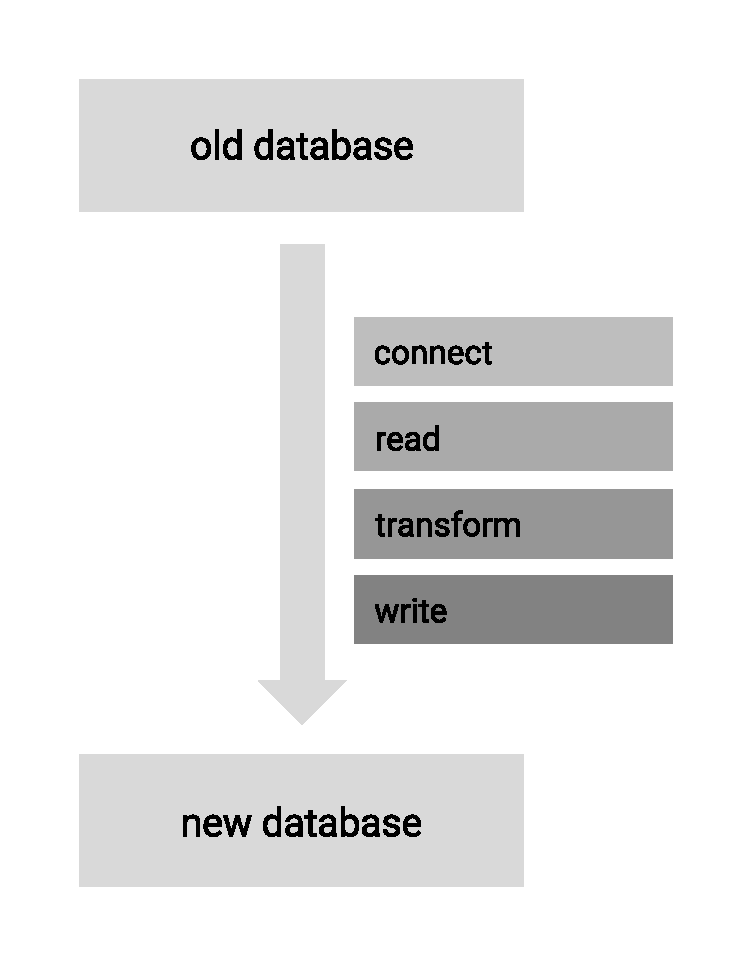
\includegraphics[width=200pt, keepaspectratio=true]{img/java-jdbm}
  \fonte{Próprio autor.}
\end{figure}

A primeira etapa da aplicação é constituída pela classe \verb|DbConnector|, que busca realizar uma conexão com um banco de dados. Para isso, ela recebe um arquivo de extensão \verb|Property| como parâmetro, que contém as credenciais necessárias para a conexão com um banco. A classe foi feita de modo genérico, sendo que é possível criar um objeto para conectar-se tanto com o banco de dados original quanto o do novo sistema, e métodos de conexão do JDBC foram utilizados em seu desenvolvimento.

A etapa seguinte corresponde à leitura dos dados do banco original, sendo realizada pela classe \verb|DbReader|. \textit{Queries} para a leitura de todas as tabelas presentes no banco original (por exemplo, \verb|select * from EVENT|) foram codificadas, e os resultados dessas \textit{queries} é obtido por meio de objetos do tipo \verb|ResultSet|. Esses objetos foram então mapeados para objetos do tipo \verb|Table|, que correspondiam às tabelas do antigo banco de dados. A classe \verb|Table| é constituída de um \verb|Set| de objetos do tipo \verb|Row|, e tanto \verb|Table| quanto \verb|Row| foram criados para armazenar os dados lidos de acordo com a tabela correspondente e, posteriormente, passá-los para a próxima etapa da \textit{pipeline}.

A terceira etapa consiste na transformação dos dados lidos para se adequarem às tabelas do banco de dados do novo projeto. O \verb|DbTransformer| foi desenvolvido para receber o conjunto de objetos do tipo \verb|Table| correspondente às tabelas do antigo banco, e transformar os dados recebidos de acordo com as tabelas no novo sistema, que diferiam do sistema original por meio da adição e/ou remoção de algumas colunas, por exemplo. Dessa forma, o \verb|DbTransformer| é constituído de outros objetos, como \verb|EventTransformer| ou \verb|BudgetTransformer|, e cada um deles retorna objetos do tipo \verb|Set| contendo uma interface construída para armazenar os dados transformados, a \verb|SQLWritable|.

Finalmente, a última etapa da \textit{pipeline} de migração do dados é responsável por conectar-se ao banco do novo sistema e escrever as \textit{queries} para a inserção dos dados transformados. Para realizar a conexão, foi utilizada uma instância do \verb|DbConnector| com um arquivo \verb|Property| com os dados do banco do novo sistema, e a interface \verb|SQLWritable| teve o método \verb|toSQL()| implementado em cada uma de suas instâncias. Esse método era responsável por escrever as \textit{queries} para a inserção dos dados de cada uma das tabelas lidas para as novas tabelas.

No desenvolvimento do AC-JDBM foram utilizados diversos conceitos de orientação a objetos, de padrões de projeto e boas práticas de programação.  A criação do projeto como uma \textit{pipeline}, a manipulação de interfaces ao invés de tipos concretos, o encapsulamento dos dados e a separação de responsabilidades pelas classes ao longo do projeto são algumas das características que contribuíram não só para o sucesso da aplicação, mas também para o aprendizado do autor na utilização da linguagem Java aplicada ao \textit{backend} de sistemas.

\section{Desenvolvimento de interfaces e experiências de usuário}
\label{sec:ui-ux-atividades}

A ser escrita.
\chapter{Conclusão}
\label{cap:conclusao}

\phantompart
\postextual
\bibliography{relatorio}

\end{document}
